%
% teil3.tex -- Beispiel-File für Teil 3
%
% (c) 2020 Prof Dr Andreas Müller, Hochschule Rapperswil
%
% !TEX root = ../../buch.tex
% !TEX encoding = UTF-8
%
\section{Die zwei grossen Theoreme
	\label{ct:section:theoreme}}
\rhead{Die zwei grossen Theoreme}
Die in diesem Kapitel untersuchten Konzepte drehen sich um das Zusammenspiel von drei Transformationen: die Radon-Transformation, die Fourier-Transformation und die Rückprojektionstransformation.

\subsection{Das Zentralschnitt-Theorem
	\label{ct:subsection:zentralschnitt}}
Das Zusammenspiel zwischen der Fourier-Transformation und der Radon-Transformation wird durch eine Gleichung erfasst, die als Zentralschnitt-Satz (oder zentraler Projektionssatz) bekannt ist. Dabei stehen $\mathscr{F}$ und $\mathscr{F}_2$ für die 1- bzw. 2-dimensionalen Fourier-Transformationen, während $\mathscr{R}$ die Radon-Transformation bezeichnet. Die Funktion $f$, die z.B. eine Dämpfungskoeffizientenfunktion darstellt, ist eine Funktion 2-dimensionaler kartesischer Koordinaten.
Beim Zentralschnitt-Theorem wird die Variable $t$ der Radon-transformierten Dämpfungskoeffizientenfunktion, welche in den Polarkoordinaten ($t, \theta$) gegeben ist, Fourier-transformiert mit $\mathscr{F}$. 
Hingegen wirkt sich die zwei-dimensionale Fouriertransformation  $\mathscr{F}_2$ auf die Euklidschenkoordinaten ($x, y$) aus.

\begin{satz}
Das Zentralschnitt-Theorem besagt, dass für jede geeignete Funktion $f$ in der Ebene und alle reellen Zahlen $S$ und $\theta$ gilt, dass
	\begin{equation}\label{2dFourier1}
		\mathscr{F}_2f(S\cos(\theta), S\sin(\theta)) = \mathscr{F}(\mathscr{R}f)(S, \theta),
	\end{equation}
\end{satz}

Im nachfolgenden wird der Beweis des Zentralschnitt-Satzes durchgeführt. 
\begin{proof}[Beweis]
	Gegeben ist die Funktion $f$, die in der Ebene definiert ist. Die reellen Zahlen $S$ und $\theta$ sind gegeben und somit ergibt sich durch die 2-dimensionale Fourier-Transformation, dass
	\begin{equation}\label{2dFourier2}
		\mathscr{F}_2(S\cos(\theta), S\sin(\theta)) = \int_{-\infty}^{\infty}\int_{-\infty}^{\infty} f(x, y)e^{-iS(x\cos(\theta)+y\sin(\theta))} \,dx\,dy.
	\end{equation}
	
	Anstatt getrennte Integrationen über die Bereiche von $-\infty < x < \infty $ und $-\infty < y < \infty$ durchzuführen, können die Punkte in der $x$-$y$-Ebene auf der Grundlage des Wertes von $x\cos(\theta) + y\sin(\theta)$ neu angeordnet werden. Genauer gesagt, werden alle Punkte $(x, y)$ in der Ebene zusammengefasst, bei denen $x\cos(\theta) + y\sin(\theta)$ gleich einer bestimmten reellen Zahl $t$ ist. Diese Gruppierung definiert genau die Gerade $l_{t,\theta}$. Ausgehend von der vorherigen Analyse erfüllt für jeden Punkt $(x, y)$ auf $l_{t,\theta}$ die reelle Zahl s, gegeben durch $s = -x\sin(\theta) + y\cos(\theta)$, die Gleichungen $x = t\cos(\theta) - s\sin(\theta)$ und $y = t\sin(\theta) - s\cos(\theta)$. Darüber hinaus, ergibt die Determinante der Matrix \begin{equation}
		\begin{bmatrix} \partial x / \partial t & \partial x /\partial s \\
			\partial y /\partial t & \partial y /\partial s \end{bmatrix} = 1,
	\nonumber \end{equation}
	 so dass $ds\,dt = dx\,dy$.
	Werden diese Anpassungen angewendet, führt dies dazu, dass die rechte Seite der Gleichung \eqref{2dFourier1} zu
	\begin{equation}\label{2dFourier3}
		\int_{-\infty}^{\infty}\int_{-\infty}^{\infty} f(t\cos(\theta) - s\sin(\theta), t\sin(\theta) - s\cos(\theta))e^{-iSt}\,ds\,dt
	\end{equation}
	wird. Der Faktor $e^{-iSt}$ kann aus der Integration herausgenommen werden, da dieser nicht von $s$ abhängt und somit wird aus \eqref{2dFourier3}
	\begin{equation}\label{fourier2radon}
		\int_{-\infty}^{\infty} \left(\int_{-\infty}^{\infty} f(t\cos(\theta) - s\sin(\theta), t\sin(\theta) - s\cos(\theta))ds\right) e^{-iSt}\,dt.
	\end{equation}
	Das innere Integral ist die Definition der Radon-transformierten Funktion $\mathscr{R}f(t, \theta)$ ausgewertet am Punkt (x, y). Das bedeutet, dass \eqref{fourier2radon} gleich ist wie
	\begin{equation}\label{radon}
		\int_{-\infty}^{\infty} (\mathscr{R}f(t, \theta)) e^{-iSt}\,dt.
	\end{equation}
	Das Integral aus \eqref{radon} ist schliesslich die Definition der Fourier-Transformation von $\mathscr{R}f$ ausgewertet bei $(S, \theta$), was also zu
	\begin{equation}\label{fourier1radon}
		\mathscr{F}(\mathscr{R}f(t, \theta))
	\end{equation}
	führt. Wie beabsichtigt, konnte die Gleichheit 
	\begin{equation}
		\mathscr{F}_2f(S\cos(\theta), S\sin(\theta)) = \int_{-\infty}^{\infty}\int_{-\infty}^{\infty} f(x, y)e^{-iS(x\cos(\theta)+y\sin(\theta))}\,dx\,dy.
	\end{equation}
	erfolgreich nachgewiesen werden.
\end{proof}

Dieser Glättungseffekt kann man in der Abbildung \ref{ct:fig:bp} gut erkennen. In dieser Abbildung können gewisse Artefakte in Form von Linien zusätzlich noch gesehen werden.

Eine einfache Visualisierung des Zentralschnitt-Theorems wird nun folgen. Bei der Fourier-Transformation der Datenpunkte, die durch das Röntgengerät aus der Radon-Transformation erhalten worden sind, werden im Wesentlichen eine Gerade im Frequenzbereich von f(x, y) auftragen. Dies kann in der Abbildung \ref{ct:img:central-slice} gesehen werden. 
Die Änderung von $\theta$, die durch Drehen des CT-Geräts zur Aufnahme von Röntgenbildern aus verschiedenen Winkeln erreicht wird, führt zur Vervollständigung weiterer Geraden im Frequenzraum. Die schrittweise Anhäufung einer ausreichenden Anzahl von Punkten ermöglicht die Extrapolation des gesamten Frequenzraums und erleichtert die Erstellung eines Bildes für $f(x, y)$ \cite{ct:condensate}.
\begin{figure}
	\centering
	\subfigure[]{\label{ct:fig:central-slice}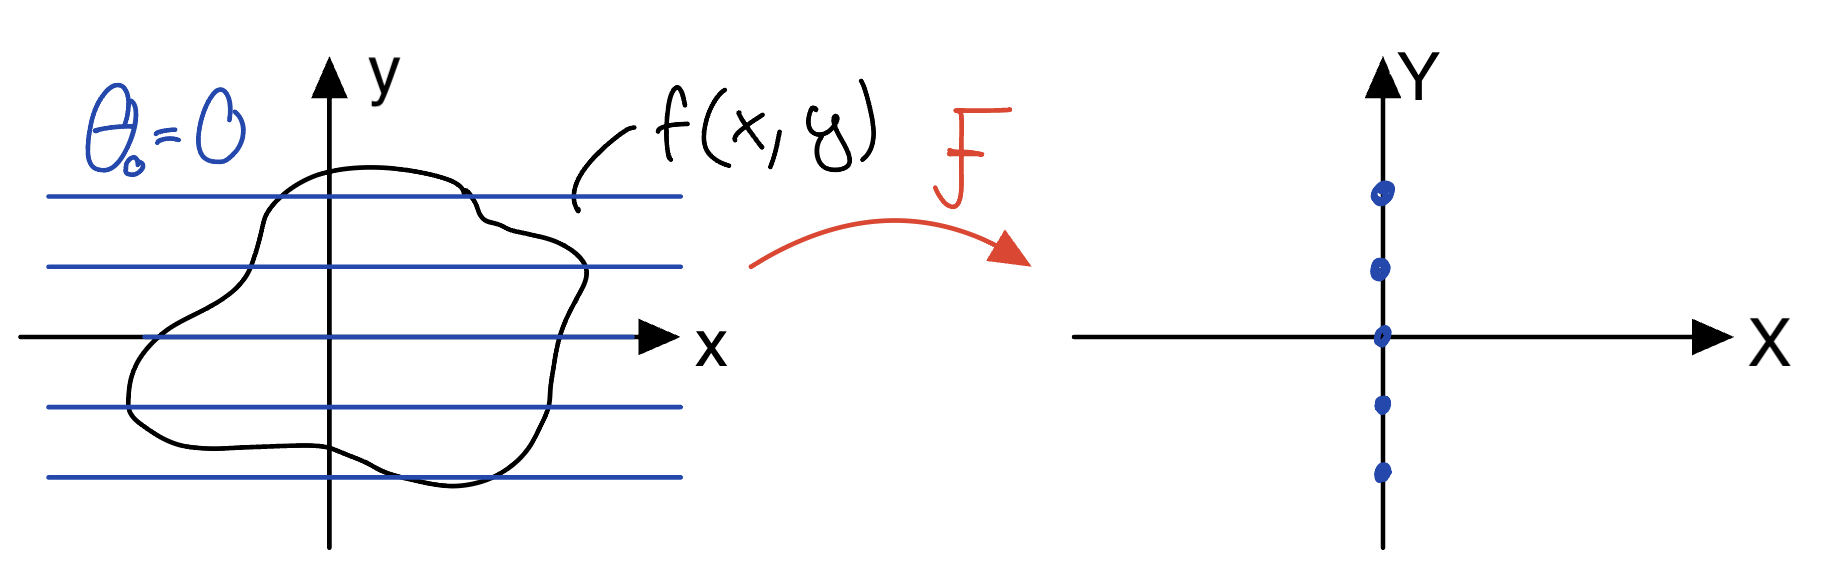
\includegraphics[width=0.35\linewidth]{papers/ct/images/central-slice.png}}
	\subfigure[Beispielbild Radon-transformiert.]{\label{ct:fig:central-slice2}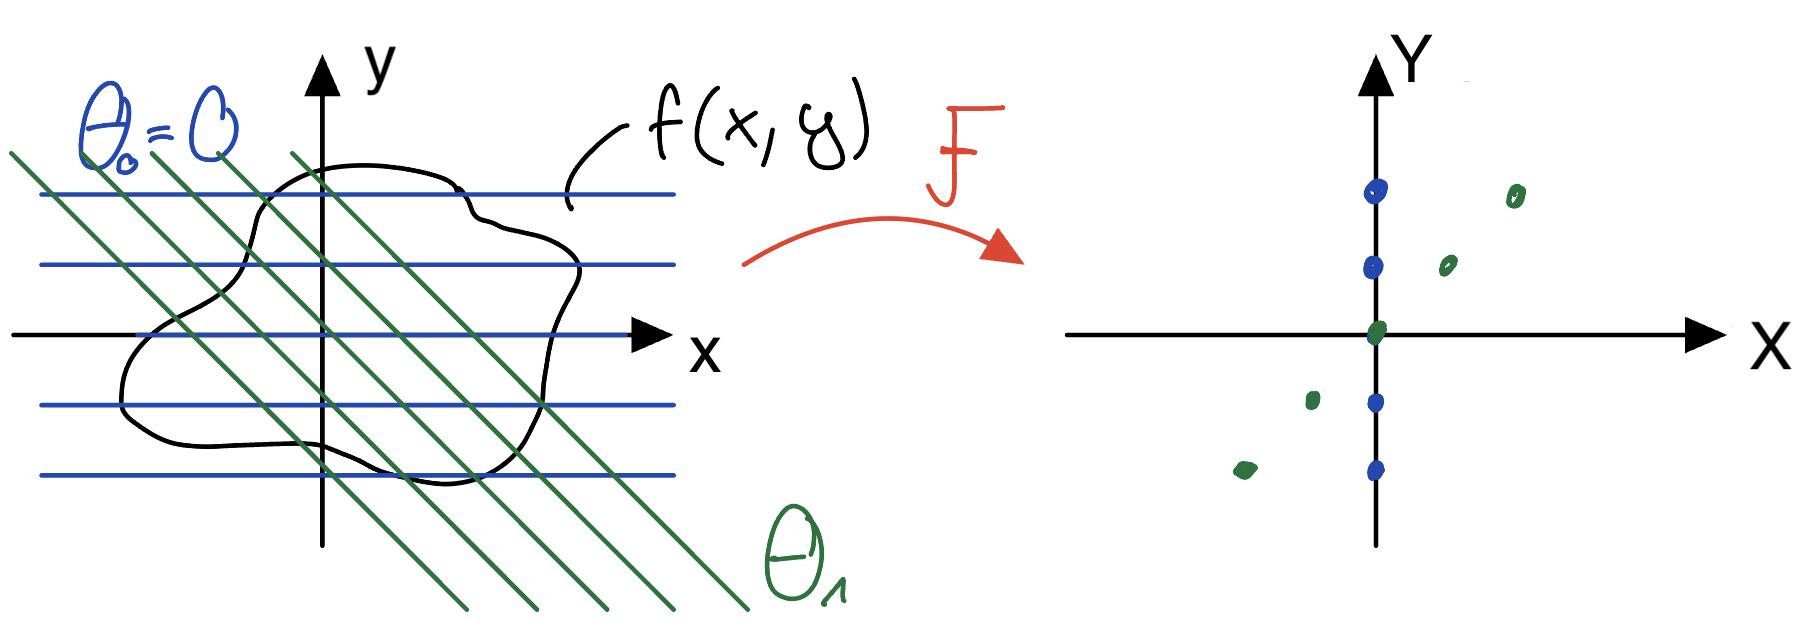
\includegraphics[width=0.55\linewidth]{papers/ct/images/central-slice2.png}}
	\caption{Visualisierung des Zentralschnitt-Theorems.}
\end{figure}


\subsection{Die gefilterte Rückprojektion
	\label{ct:subsection:gefilterterueck}}
Die Rückprojektion diente als erster Versuch, die Radon-Transformation zu invertieren und die Funktion des Dämpfungskoeffizienten zu ermitteln. Das Ergebnis war jedoch eine geglättete Version der ursprünglichen Funktion und keine exakte Übereinstimmung. Das nachfolgende Theorem, das als gefilterte Rückprojektion bekannt ist, zeigt eine Methode zur Korrektur des Glättungseffekts und zur genauen Wiederherstellung der ursprünglichen Funktion.

Die gefilterte Rückprojektion besagt, dass für eine geeignete Funktion $f$, die in einer Ebene definiert ist und für reelle Zahlen $x$ und $y$ gilt, dass
\begin{equation}
	f(x, y) = \dfrac{1}{2}\mathscr{B}\biggl(\mathscr{F}^{-1}[|S|\mathscr{F}(\mathscr{R}f(S, \theta))]\biggr)(x,y).
\end{equation}

Als nächstes folgt der Beweis für die gefilterte Rückprojektion.
\begin{proof}[Beweis]
	Wird die (2-dimensionale) Fourier-Transformation und die Inverse-Fourier-Transformation auf eine Funktion $f$ angewendet, resultiert 
	\begin{align}\label{iftnft}
		f(x, y) &=\mathscr{F}_2^{-1} \mathscr{F}_2 f(x, y). \\
		\intertext{	Wird die Definition der inversen 2-dimensionalen Fourier-Transformation auf der rechten Seite der Gleichung angewendet, folgt dass}
				&=\dfrac{1}{4\pi^2} \int_{-\infty}^{\infty}\int_{-\infty}^{\infty} \mathscr{F}_2 f(x, y)e^{+i(xX + yY)}\,dX\,dY. \\
		\intertext{Danach wird eine Koordinaten-Transformation von Kartesischen- zu Polarkoordinaten durchgeführt, wobei $X = S\cos(\theta)$ und $Y = S\sin(\theta)$. Dabei ist $S$ auf reelle Zahlen und $\theta$ auf den Bereich $0 \le \theta \le \pi$ beschränkt. Angesichts dieser Änderung resultiert für $dX\,dY = |S|\,dS\,d\theta$, anstatt $S\,dS\,d\theta$. Dies führt dazu, dass}
				&= \dfrac{1}{4\pi^2} \int_{0}^{\pi}\int_{-\infty}^{\infty} \mathscr{F}_2 f(S\cos(\theta), S\cos(\theta))e^{+iS(x\sin(\theta) + y\sin(\theta))}\,|S|\,dS\,d\theta \\
		\intertext{	resultiert. Aus dem Zentralschnitt-Satz folgt für den Integrand $\mathscr{F}_2 f(S\cos(\theta), S\cos(\theta))$, dass dies das Gleiche ist wie $\mathscr{F}(\mathscr{R}f)(S, \theta)$. Somit kann auch geschrieben werden, dass}
				&= \dfrac{1}{4\pi^2} \int_{0}^{\pi}\int_{-\infty}^{\infty} \mathscr{F}(\mathscr{R}f)(S, \theta)e^{+iS(x\sin(\theta) + y\sin(\theta))}\,|S|\,dS\,d\theta.\\
		\intertext{Das innere Integral in Bezug auf $S$ ist definiert, als das $2\pi$-fache der inversen Fourier-Transformation der Funktion $|S|\mathscr{F}(\mathscr{R}f)(S, \theta)$ ausgewertet am Punkt $(x\cos(\theta) + y\sin(\theta), \theta)$. Dies führt dazu, dass }
				&= \dfrac{1}{2\pi} \int_{0}^{\pi} \mathscr{F}^{-1}[|S|\mathscr{F}(\mathscr{R}f)(S, \theta)](x\cos(\theta)+y\sin(\theta), \theta)\,d\theta.\\
		\intertext{\sloppy Dies ist wiederum das Integral, welches auch für die gefilterte Rückprojektion der Funktion $\mathscr{F}^{-1}[|S|\mathscr{F}(\mathscr{R}f(S, \theta))]$ verwendet wird. Deshalb entspricht auch}
		f(x, y) &= \dfrac{1}{2}\mathscr{B}\biggl(\mathscr{F}^{-1}[|S|\mathscr{F}(\mathscr{R}f(S, \theta))]\biggr)(x,y),
	\end{align}
	womit die gefilterte Rückprojektionsformel erfolgreich eingeführt wurde.
\end{proof}

Würde in der Formel der Faktor $|S|$ fehlen, würden sich die Fourier-Transformation und ihre Umkehrung gegenseitig aufheben, so dass nur die Rückprojektion der Radon-Transformation von $f$ übrig bliebe. Wenn man die 1-dimensionale Fouriertransformierten für verschiedene Winkel aufaddiert, dann werden bei tiefen Frequenzen viele Werte zusammengezählt, bei hohen Frequenzen nur wenige. Dieser Effekt wird ausgeglichen durch Multiplikation mit dem Betrag der Frequenz entlang der Frequenzachse $\omega$. Das entscheidende Element in der Formel besteht also darin, die Fourier-Transformierte von $\mathscr{R}f(S, \theta)$ mit der Absolutwertfunktion $|S|$ zu multiplizieren, bevor die inverse Fourier-Transformation durchgeführt wird. Im Kontext der Signalverarbeitung wird die Fourier-Transformation von $\mathscr{R}f$ als gefiltert durch Multiplikation mit $|S|$ beschrieben. Genau aus diesem Grund wird die Formel auch als \glqq gefilterte Rückprojektionsformel\grqq{} bezeichnet.

Die Formel für die gefilterte Rückprojektion dient als Basis der Bildrekonstruktion. Sie beruht jedoch auf der Annahme, dass die Werte von $\mathscr{R}f(S, \theta)$ für alle möglichen Geraden $l_{S, \theta}$ bekannt sind. In der Praxis ist dies nicht möglich, da nur eine endliche Anzahl von Röntgenproben genommen wird und ein Bild aus den gesammelten Daten approximiert werden muss. Folglich gibt es für jede endliche Menge von Röntgenstrahlen, die einen Scan bilden, von Null abweichende Dämpfungskoeffizientenfunktion, die als Artefakte bezeichnet werden und deren Radon-Transformationen für alle Zeilen des Scans zu Null werden.




















